% ****** Start of file apssamp.tex ******
%
%   This file is part of the APS files in the REVTeX 4.2 distribution.
%   Version 4.2a of REVTeX, December 2014
%
%   Copyright (c) 2014 The American Physical Society.
%
%   See the REVTeX 4 README file for restrictions and more information.
%
% TeX'ing this file requires that you have AMS-LaTeX 2.0 installed
% as well as the rest of the prerequisites for REVTeX 4.2
%
% See the REVTeX 4 README file
% It also requires running BibTeX. The commands are as follows:
%
%  1)  latex apssamp.tex
%  2)  bibtex apssamp
%  3)  latex apssamp.tex
%  4)  latex apssamp.tex
%
\documentclass[%
 % reprint,
10pt,
superscriptaddress,
twocolumn,
%groupedaddress,
%unsortedaddress,
%runinaddress,
%frontmatterverbose,
%preprint,
%preprintnumbers,
%nofootinbib,
%nobibnotes,
%bibnotes,
 amsmath,amssymb,
 aps,prx,
%pra,
%prb,
%rmp,
%prstab,
%prstper,
%floatfix,
]{revtex4-2}

\usepackage{graphicx}% Include figure files
\usepackage{dcolumn}% Align table columns on decimal point
\usepackage{bm}% bold math
\usepackage{xcolor}
\usepackage{hyperref}% add hypertext capabilities
\usepackage{siunitx}% SI units
\newcommand{\ecoli}[0]{\textit{E. coli}} % use \ecoli command to correctly typeset italic E. coli

\graphicspath{{figures/}} % set default figure path to figures/, if we store figure files in figures/, we only need to put file name in \includegraphics{filename.pdf}

% Some formatting guidelines
% 1. Start a new line (\n) for each sentence. This is good for synctex (click pdf and find the line in tex), and also good for Git when comparing versions.
% 2. Communicate thoughts in comments. For example, if you think a figure of something is needed but missing some where, put a comment and describe the needs.
% 3. Colored text: I use red text to emphasize that the claim is not fully backed by our results. The wording may be modified in the future.
% 4. Figure crossref: at the beginning of a sentence, use "Figure~\ref{}". Otherwise, use "Fig.~\ref{}". Note that the "~" is to prevent line breaking in the middle of the crossref.

% Some content problems that need to be fixed
% 1. Same quantities are referred to in different notations, e.g. \tau^* and \tilde{\tau}, x and y, \tilde{D} and D_A



\begin{document}

\preprint{APS/123-QED}

\title{Bacterial Dynamics in Curved Spaces}% Force line breaks with \\

\author{Cristian Villalobos Concha}
\author{Maria Luisa Cordero}
\author{Rodrigo Soto}
\affiliation{Departamento de Física, FCFM, Universidad de Chile, Santiago, Chile.}

% \altaffiliation[Also at ]{Laboratoire Gulliver, UMR 7083 CNRS, ESPCI Paris, PSL Research University, 75005 Paris, France.}%Lines break automatically or can be forced with \\
\author{Anke Lindner}
\author{Eric Clément}
\affiliation{%
 Laboratoire PMMH, UMR 7636 CNRS-ESPCI-Sorbonne Université-Université Paris Diderot, 7-9 quai Saint-Bernard, 75005 Paris, France.
 }%

\author{Teresa Lopez-Leon}

\affiliation{Laboratoire Gulliver, UMR 7083 CNRS, ESPCI Paris, PSL Research University, 75005 Paris, France.}
\date{\today}
% It is always \today, today,
%  but any date may be explicitly specified
\author{Zhengyang Liu}

\affiliation{%
 Laboratoire PMMH, UMR 7636 CNRS-ESPCI-Sorbonne Université-Université Paris Diderot, 7-9 quai Saint-Bernard, 75005 Paris, France.
 }%
\affiliation{Laboratoire Gulliver, UMR 7083 CNRS, ESPCI Paris, PSL Research University, 75005 Paris, France.}

\begin{abstract}
The interplay between complex environments and active matter suggests a possibility to control and engineer active matter by carefully designing the confinement structures.
It is now well established that confinement may influence transport, rheology, pressure, spatial distribution and collective motion of active matter.
Curved confining walls, which are ubiquitous in biological systems, show their own, specific rich and intriguing effects on active matter.
Here, using a double emulsion system, where the inner and outer droplet sizes can be independently controlled, we experimentally investigate the influence of curved confinement on an active bath of \textit{Escherichia coli} (\ecoli) bacteria.
In particular, we analyze the fluctuations of the inner droplet using the framework of a stochastic ``active noise'' model, and show that the strength of active noise is not an intrinsic property of an active bath, but depends on the confinement curvature.
\textcolor{red}{Our numerical simulations revealed the origin of this dependence on confinement.}
Our results pose new challenge to active matter theory and suggest new methods to control active matter.

\end{abstract}

%\keywords{Suggested keywords}%Use showkeys class option if keyword
                              %display desired
\maketitle

\section{Introduction}
% Use "Active noise" key word to label all the literatures related to this project
The interactions between active and passive objects are always intriguing.
On the one hand, passive objects are often used as a probe to assess the properties, in particular activity, which are sometimes challenging to measure directly.
On the other hand, the capabilities of activity to ehance mixing of fluids and transport of nutrients show great ecological significance and can potentially enable important biomedical applications \cite{Kurtuldu2011, Pushkin2013, Saintillan2008a, Sokolov2009a}.

On the most elementary level, the interaction between an active particle and a passive particle can be described as ``scattering''.
In this process, the active particle swims by the passive particle results in a closed-loop trajectory, due to the hydrodynamic head-rear symmetry of the model swimmer \cite{Dunkel2010}.
In the presence of a confining wall, the flow field generated by an active swimmer is modified, as if there is a mirror image of the swimmer, with force singularities pointing in opposite directions \cite{Blake1974}.
The head-rear symmetry is broken in the modified flow field, leading to net displacement of passive object in a single scattering event.
Based on this picture, Mino et al. successfully modeled the confinement effect on the diffusivity of passive particles in active bath \cite{Mino2011, Mino2013}.
\citet{Lagarde2020} focused their experiment more on the single scattering event, and found far field hydrodynamic interactions to be irrelevant compared to direct collisions.
The experiments mentioned above all revealed an important aspect of active baths: the effect on passive tracer diffusivity is stochastic and additive.
This discovery has led to efforts to model active baths as a stochastic noise \cite{Gregoire2001, Maggi2014, Wu2000, Ye2020}.

Boundaries are known to have dramatic impact on active matter, with examples of pattern formation, directed flow and unusual mechanical properties \cite{Wioland2013, Wu2017, Liu2019}.
Planar boundaries, which are common and easy to produce in labs, have been studied extensively in the past two decades.
However, less is known about how curved boundaries affect active matter behavior.

In this paper, we experimentally investigate this question by putting active bacterial suspensions into the middle layer (also know as the ``shell'' layer) of oil-water-oil double emulsions.
We analyze the fluctuations of the inner droplet using the framework of a stochastic ``active noise'' model, and show that the strength of active noise is not an intrinsic property of an active bath, but depends on the confinement curvature.
\textcolor{red}{Furthermore, we show that the dependence on confinement originates from two aspects: collision angle and activity. Our numerical simulations reveal the origin how spherical confining wall reduces the activity of an active bath.}
Our results deepen the understanding of active matter behavior under confinement.

\section{Experiment}
% Initial version is copied from Overleaf

\begin{figure*}[!t]
  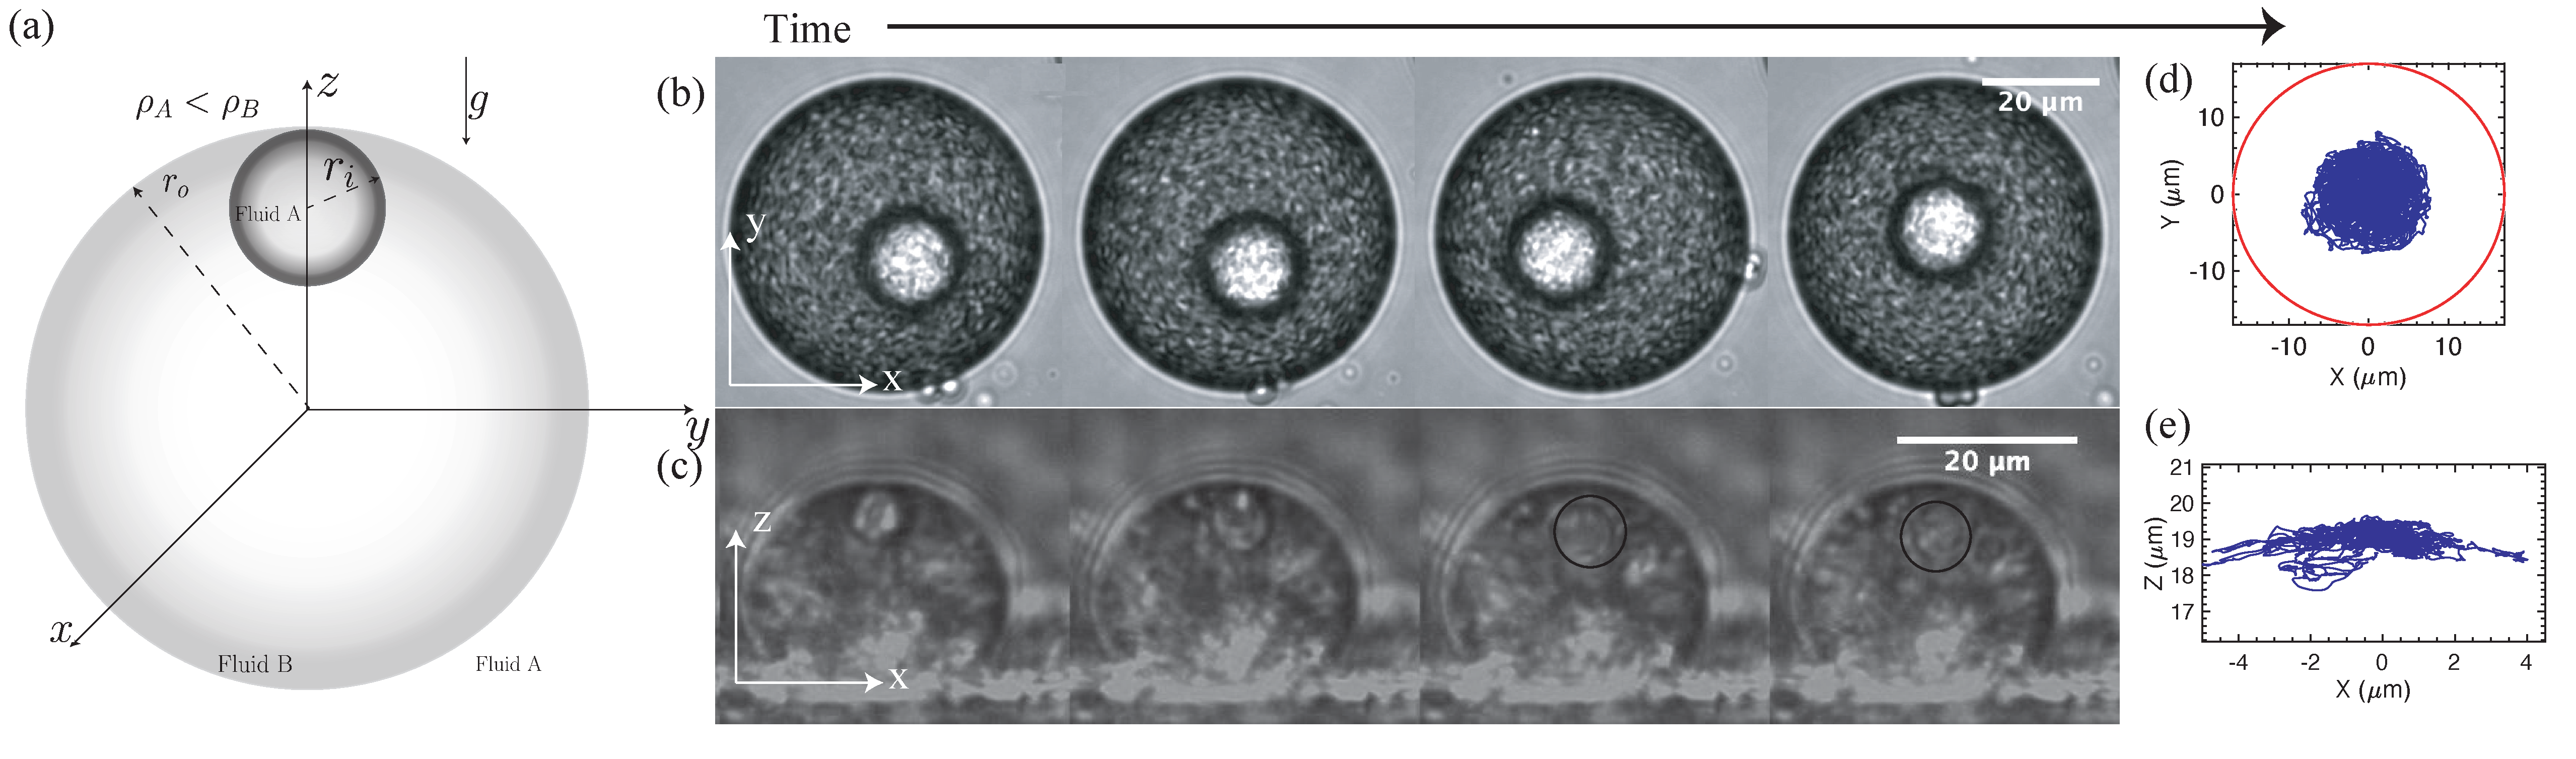
\includegraphics[width=\textwidth]{Diagrama_DE}
  \caption{
  \textbf{Double emulsion --- bacterial shells.}
  (a) A Schematic diagram of the bacterial shell system, along with the coordinate system defined on it.
  The outer droplet of density $\rho_A$ and radius $r_o$ filled with bacterial suspensions.
  Inside this droplet there is another droplet filled with an oil of density $\rho_B < \rho_A$.
  (b) Sequence of image separated by $\Delta t =\SI{5}{\second}$. Top row; shows the XY plane of a bacterial shell of outer diameter $r_o=\SI{27}{\micro\meter}$ and a inner droplet of diameter $r_i=\SI{13.5}{\micro\meter}$.
  (c) A view of the XZ plane of a drop of diameter $r_o=\SI{11.5}{\micro\meter}$ and a inner drop of $r_i=\SI{2.9}{\micro\meter}$.
  (d-e) Trajectory of the center of the inner droplet.
  }
  \label{montaje_doble}
\end{figure*}

Bacterial Culture:
Here we used wild-type e.coli bacteria (strain  W3110). The bacteria were grown with a standard culturing protocol, 10 $\mu L$ of frozen stock stored at -20 degrees is  diluted  in 10 $mL$ of lysogenic broth (LB) and putted on a shaker at  temperature 30º, and 210 rpm overnight. The saturated culture is diluted in a proportion of $1:100$ in LB medium and let it grow until the mid-log phase of growth, which is equivalent to a optical density ($OD_{600}$) $\approx$ 0.6. Cells were harvested at 2100 $g$ for 10 min. Then the supernatant is removed, and the pellet is resuspended in minimal motility buffer (MMA).  This allows the bacteria to swim but do not divide.  A volume of $10 \mu L$ is added in $1 mL$ of Hexadecane containing 2% weight Span 80 as a surfractant. The mixture is mannually agitated and the diluted 1:10 in 1 mL of Hexadecane. Then 200 $uL$ of the emulsion is putted in a square observation chamber of $L = 1 cm$  and height $h=400\mu m$. The chamber are fabricated in a SU-8 photoresist (Gersteltec GM 1075) with optical lithography on a 50.8 $mm$ diameter glass wafer.

In this work, we study the agitation due to a suspension of bacteria \textit{E.coli} confined on a double emulsion-bacterial shell shown in Fig.~\ref{montaje_doble}.

The bacterial suspension is encapsulated in a double emulsion, where an oil droplet gets trapped inside a water-in-oil emulsion.
We show that the inner oil droplet performs a persistent random walk for short times and a saturation regime for large times.
The bacteria used is a wild-type \ecoli~(RP437)  which contains a plasmid to express the green fluorescence protein (GFP), and  \ecoli~(W3110) which is also genetically modified to express the green fluorescence protein (GFPmut2).  Both strains have the same features (e.g., run and tumble), but the difference is how they express the GFP.

The bacteria were grown using a standard protocol, washed, and re-suspended in a motility medium, allowing the bacteria to swim but not divide.
The final concentration of the bacterial suspension ranges from $OD_{600} = 0.7$ to $OD_{600} = 150$.
A volume of 10 $\mu$L of the bacterial suspension is added to 1 mL of hexadecane containing 2 wt\% Span 80 (Sigma-Aldrich, S6760) as a surfactant.
The mixture is manually shacking, resulting in an emulsion of aqueous droplets containing the bacterial suspension in oil; also, less commonly, bacterial droplets will form with a drop of oil inside, i.e. a double emulsion.
The observation setup is a square chamber of inner side $L = 1$ cm and height $h = 400$ $\mu$m. The chamber walls are fabricated in SU-8 photoresist (Gersteltec GM 1075) with optical lithography (Heidelberg Instruments MLA 100) on a 50.8 mm diameter and 500 $\mu$m thick circular glass wafer.
As the aqueous bacterial suspension is denser than the ambient hexadecane, drops sediment to the bottom of the chamber.
The inner droplet rises by the buoyancy to the top of the bacterial droplet.
For the measurements in the XY plane, the chamber is placed on an inverted microscope (Nikon TS100F), observed with a 60X objective, and filmed at 10--100 Hz.
For the XZ plane, when the emulsion is made, it is collected into a 1 mm square capillary and observed using an inverted confocal microscope with a 40X objective, filming at 50--70 Hz with a camera mounted on the microscope.
Besides, the confocal microscope can be rotated, which allows us to observe the drops from the side instead of the top-bottom sight.
In Fig.~\ref{montaje_doble}(a), we show the coordinates defined on the double emulsion, where Fluid A is hexadecane, and fluid B is the bacterial suspension.
The inner droplet moves randomly due to the bacterial suspension [Fig.~\ref{montaje_doble}(b)], without the bacterial suspension, due to the size of the internal drop, it would not be able to move due to thermal fluctuations.
In the bottom row of Fig.~\ref{montaje_doble}(b), we can see that the inner droplets remain in the top part of the droplet.

\section{1D model}
% I rewrite the 1D model part based on the overleaf version to serve as a reference for the discussions of the results.

To model the experiment, we consider the inner droplet as a passive particle agitated by an active noise.
The outer droplet imposes confinement on the inner droplet.
For a small displacement from the equilibrium point, the effect of the curved surface can be approximated by a harmonic potential.
The equation of motion for the inner droplet in the Low Reynolds number limit is the overdamped Langevin equation:
%
\begin{align}
    \label{eq.Langevin}
    \dot{x}=u(t)-\frac{x}{\tilde{\tau}}.
\end{align}
%
where $\tilde{\tau}=\Gamma/k$, with $\Gamma$ the friction coefficient, $k$ the spring constant for the harmonic potential, and $u(t)$ is the active noise induced by the bacterial suspension.
We will model the active noise as a colored Gaussian noise, with the following statistical properties:
%
\begin{align}
    \label{eq.act.noise}
    \langle u(t)\rangle &=0,\\
    \langle u(t)u(t')\rangle &=\frac{\tilde{D}}{\tau}e^{-|t-t'|/\tau}.
\end{align}
%
where $\tilde{D}$ is the active diffusion coefficient, and $\tau$ is the persistence time of the bacterial fluxes. The solution of the eq(\ref{eq.Langevin}) is given by:
%
\begin{align}
    \label{sol:langevin}
    x(t) = x_oe^{-t/\tilde{\tau}}+\int_{0}^{\infty}ds e^{-|t-s|/\tilde{\tau}}u(s).
\end{align}

We can derive the mean-square displacement (MSD):
%
\begin{align}
    \label{eq.MSD_1d}
    \langle \Delta x^2(t)\rangle = \frac{2(\tilde{D}/\tau)}{\frac{1}{\tilde{\tau}}+\frac{1}{\tau}}\left(\frac{1-e^{-\frac{2t}{\tilde{\tau}}}}{\frac{2}{\tilde{\tau}}}-\frac{e^{-(\frac{1}{\tilde{\tau}}+\frac{1}{\tau})t}-e^{-\frac{2t}{\tilde{\tau}}}}{\frac{1}{\tilde{\tau}}-\frac{1}{\tau}}\right),
\end{align}
%
with the short and long time limits given by:
%
\begin{align}
    \label{eq.limits}
    \lim_{t\to0} \langle \Delta x^2(t)\rangle & = \frac{\tilde{D}}{\tau}t^2,\\
    \lim_{t\to\infty} \langle \Delta x^2(t)\rangle & =\frac{\tilde{D}(\tau^*)^2}{\tilde{\tau}+\tau}.
\end{align}
%
We can see that the MSD is ballistic at short times andsaturates to a constant value at long times due to the confinement imposed by the harmonic potential. In Fig.~\ref{fig:msd-1d-model} we show two plots of the Eq.~\ref{eq.MSD_1d} for different values of $\tilde{\tau}$ while keeping $\tau$ fixed, and different $\tau$ while keeping $\tilde{\tau}$ fixed.

\begin{figure}
  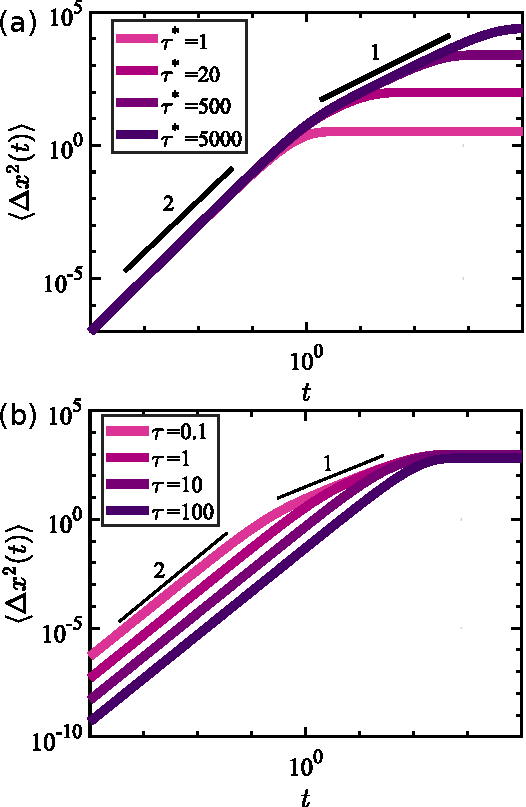
\includegraphics[width=\columnwidth]{model-msd-illustration}
  \caption{
  \textbf{MSD 1D model.}
  (a) Different values of $\tilde{\tau}$, where $\tau=0.5$ and $D=5$.
  (b) Different values of $\tau$, where $\tilde{\tau}=200$ and $D=5$.
  }
  \label{fig:msd-1d-model}
\end{figure}

\section{Results}

\subsection{Inner droplet trajectories}

In the double emulsion experimental system, the inner droplet is frequently ``kicked'' by the many swimming bacteria around it.
As a result, it exhibits fluctuations much stronger than Brownian motion in the horizontal ($y$) direction.
Due to the smaller density of the inner droplet relative to the bacterial suspension, a buoyant force is constantly pushing it to the top surface of the outer droplet, making the dome an equilibrium position.
In the vertical ($z$) direction, the inner droplet mostly follows the outer droplet surface.
A typical inner droplet trajectory is shown in Fig.~\ref{fig:traj-analysis}(a).
The colored dots denote the positions of inner droplet center at different time.
In cases where inner droplet size is very small, while the bacterial activity is large, inner droplet can leave the surface.
We can roughly estimate the critical inner droplet radius, below which bacterial activity can overcome buoyant force.
The buoyant force is $F_b = \frac{4}{3}\pi r_i^3\Delta\rho g$, where $\Delta\rho\approx 230$ kg/m$^3$ is the density difference between water and hexadecane, and $g\approx 9.8$ m/s$^2$ is the gravitational accelaration.
The propelling force of a single bacteria is approximated by the Stokes drag on a sphere $F_a \approx 6\pi\eta r_b V_b$, where $\eta=0.001$ Pa$\cdot$s is water viscosity, $r_b\approx 0.5$ $\mu$m is bacteria cross section radius and $V_b \approx 20$ $\mu$m/s is the simming speed of bacteria.
Let $F_b=F_a$, we get a critical droplet radius $r_c \approx 2.7$ $\mu$m.
Indeed, since we never prepared inner droplet with radius $r_i < r_c$, inner droplet leaving the surface is a rare event.
However, in very concentrated bacterial suspensions, the inner droplet can leave the surface even when $r_i > r_c$.
This is likely due to more frequent collision event, or collective motions.

\begin{figure*}[!t]
  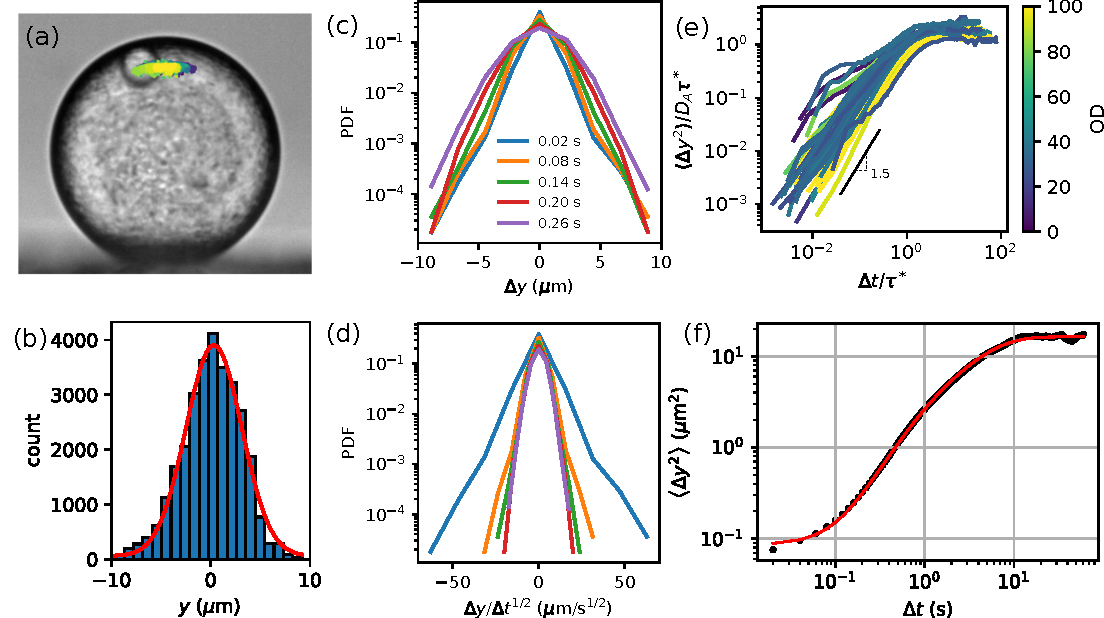
\includegraphics[width=\textwidth]{2-traj-analysis}
  \caption{
  \textbf{Inner droplet trajectory analysis.}
  (a) The trajectory of the inner droplet plotted on an experimental image.
  Outer droplet radius $r_o= 33.2$ $\mu$m and inner droplet radius $r_i=6.0$ $\mu$m.
  Color from dark purple to bright yellow denotes time from the beginning to the end.
  (b) Position probability distribution in $y$ direction. Red curve is a Gaussian fit to the distribution, with mean $\mu = -0.3$ $\mu$m and standard deviation $\sigma = 2.8$ $\mu$m.
  (c) Displacement probability density function (PDF) in $y$ direction, at various time interval $\Delta t$.
  (d) Displacement PDF, where the displacement $\Delta y$ is rescaled by the square root of time interval $\Delta t^{1/2}$.
  (e) Mean square displacement (MSD) of all inner droplet trajectories in this study, with time rescaled by fitted relaxation time $\tau^*$ and MSD rescaled by the product of active diffusivity and relaxation time $D_A\tau^*$.
  (f) A fit of MSD data to our 1D model, fitting parameters are $D_A=1.95$ $\mu$m$^2$/s, $\tau=0.25$ s, $\tau^*=4.40$ s and $c=0.086$ $\mu$m$^2$/s.
  }
  \label{fig:traj-analysis}
\end{figure*}

Next, we measured the position and displacement probability distribution functions (PDF) in the horizontal direction, as shown in Figs.~\ref{fig:traj-analysis}(b-d).
The distribution is well fitted by a Gaussian function, shown as the red curve.
According to \citet{Leptos2009}, in the presence of swimmers, the displacement PDF is characterized by a Gaussian core and exponential tails.
In our data, exponential tails are also observed when $\Delta t = 0.02, 0.08, 0.14$ s, manifesting anomalous transport [Fig.~\ref{fig:traj-analysis}(c)].
Further increasing the time interval makes the exponential tails disappear.
\textcolor{red}{When rescaling the displacement $\Delta y$ with square root of time interval $\Delta t^{1/2}$, as shown in Fig.~\ref{fig:traj-analysis}(d), we notice that all the Gaussian cores of the PDF curves, except the $\Delta t=0.02, 0.08$ s ones, collapse on the same master curve.
The deviations of the small $\Delta t$ curves from the master curve suggest that strong persistence is in play at this time scale $\tau_c\approx 0.1$ s, rather than a random diffusive process.}
Finally, we measured the mean square displacement (MSD) of inner droplets in all our experiments, at various bacterial concentrations and droplet sizes, as shown in Fig.~\ref{fig:traj-analysis}(e).
The lag time and MSD are rescaled by $\tau^*$ and $D_A\tau^*$, respectively, which are obtained from fitting the original MSD data to the 1D model described before.
An example of the fit is shown in Fig.~\ref{fig:traj-analysis}(f).
Typically, the MSD is characterized by a superdiffusive regime at small $\Delta t$, and a transition to saturation at large $\Delta t$.
A diffusive regime can be identified in some cases, but not always.
The critical $\Delta t$'s, $\tau$ and $\tau^*$, vary with droplet sizes and possibility bacterial concentrations, which will be discussed in the following section.

\subsection{Confinement effect}

We studied the motions of inner droplets in over 100 systems of various sizes and bacterial concentration.
Although the simple ``mechanical mixing'' technique does not provide accurate control over droplet sizes, we manage to explore a considerable large parameter space in detail, and to reveal the confinement effect.
The explored parameter space is shown in Fig.~\ref{fig:confinement-effect}(a).
Since we have 3 different parameters varying at the same time, we shall select experiments where two of the parameters are fixed, in order to illustrate the effect from a single parameter.
Here, we choose $\text{OD}\in(20, 40]$ (blue pentagons) and $\text{OD}\in(60, 80]$ (green squares) to illustrate low and high bacterial concentrations, respectively.
To see the effect of outer droplet radius $r_o$, we select data where $r_i\in[5, 9]$ ($\mu$m) and plot active diffusivity $D_A$, persistence time $\tau$ and relaxation time $\tau^*$ as functions of $r_o$, as shown in Fig.~\ref{fig:confinement-effect}(b).
We find that $D_A$ increases monotonically with $r_o$ at both low and high OD.
The increasing rate at high OD, characterized by the slope of $D_A$-$r_o$ curve, is much larger than that at low OD.
$\tau$ and $\tau^*$ show little to no dependence on $r_o$ in our experiments.
Similarly, to see the effect of inner droplet radius $r_i$, we select data where $r_o\in[30, 50]$ ($\mu$m) and plot $D_A$, $\tau$ and $\tau^*$ as functions of $r_i$, as shown in Fig.~\ref{fig:confinement-effect}(c).
We find that neither $D_A$ nor $\tau$ show pronounced dependence on $r_i$, while $\tau^*$ decreases monotonically with $r_i$.
Interestingly, $\tau^*$ at different OD's are quite consistent in magnitude.

% I'm not sure if I should discuss the predictions of the model here, or later in another section.

\begin{figure}[!t]
  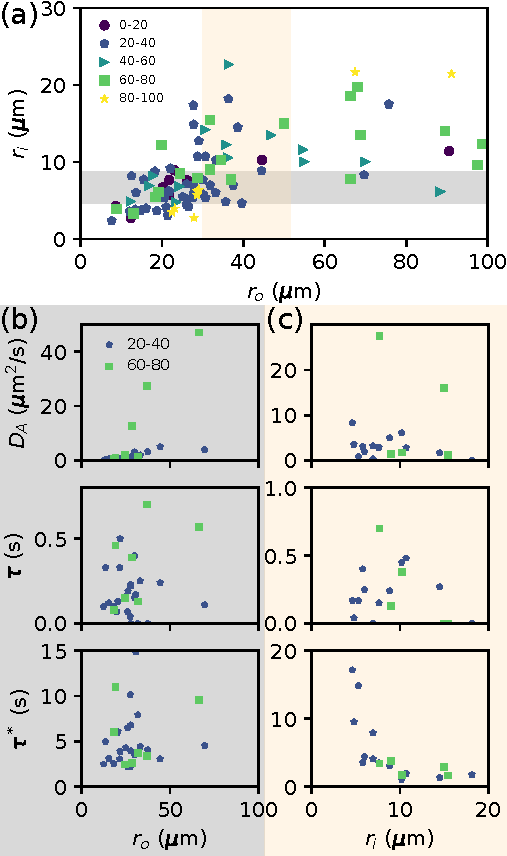
\includegraphics[width=\columnwidth]{3-confinement-effect}
  \caption{
  \textbf{Confinement effect on the inner droplet motions.}
  (a) Explored parameter space of outer droplet radius $r_o$, inner droplet radius $r_i$ and bacterial concentration in terms of optical density (OD).
  OD's are divided in 5 groups, shown as different colors and markers in the plot.
  Two bins of data are selected to highlight the confinement effect.
  The first bin is $r_i\in[5, 9]$ ($\mu$m), as shaded in gray.
  The second bin is $r_o\in[30, 50]$ ($\mu$m), as shaded in light orange.
  (b) Fitting parameters $D_A$, $\tau$ and $\tau^*$ plotted as functions of $r_o$ in the first bin.
  (c) Fitting parameters $D_A$, $\tau$ and $\tau^*$ plotted as functions of $r_i$ in the second bin.
  }
  \label{fig:confinement-effect}
\end{figure}


\subsection{Bacterial activity}

The confinement effect on the active diffusivity may be correlated with the bacterial activity.
Indeed, we frequently observed very different activity at the same bacterial concentration.
In order to quantify the activity, we perform particle image velocimetry (PIV) analysis on the bright field images of active double emulsions and use the root mean square of the PIV velocity magnitude as a measure of activity.
Formally, we obtain velocity magnitude field $\mathbb{V}=\{V_{ij}\}$ from PIV.
The mean velocity $\overline V$ is defined as
%
\begin{equation}
    \overline V = \sqrt{\frac{1}{n}\sum_{ij} V_{ij}^2}.
\end{equation}
%
To suppress noise from the detection, mean velocities are measured in each pair of frames and then averaged. In the data presented here, all the PIV analysis are performed with OpenPIV (version 0.24.2). We fix the interrogation window size at 20 pixels throughout all the analyses, with overlap between adjacent windows at 10 pixels.

\begin{figure}[!t]
  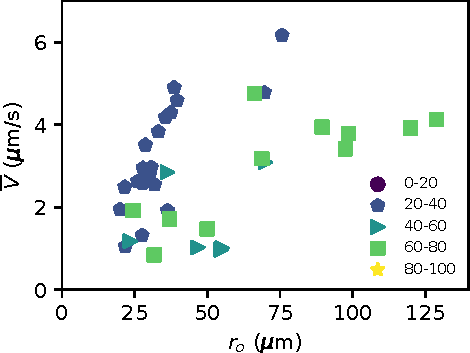
\includegraphics[width=\columnwidth]{bacterial-activity}
  \caption{
  Mean PIV velocity $\overline V$ as a measure of bacterial activity, plotted against outer droplet radius $r_o$.
  }
  \label{fig:bacterial-activity}
\end{figure}

In Fig.~\ref{fig:bacterial-activity}, we plot $\overline V$ as a function of $r_o$.
As usual, the data are put into different groups by bacterial concentrations.
In each OD bin, in particular $\text{OD}\in(20, 40]$ (blue pentagons) and $\text{OD}\in(60, 80]$ (green squares), $\overline V$ increases with $r_o$, suggesting that droplet confinement hinders the activity of bacteria.
However, from this data, it is still unclear how activity depends on OD.

\textcolor{red}{
At the moment, we have not finished PIV on all the videos, partially due to the less organized data analysis in the past.
As a result, we see less data points in Fig.~\ref{fig:bacterial-activity} compared to the parameter space plot Fig.~\ref{fig:confinement-effect}(a).
In addition, I did not have Cristian's raw data from Chile, so it was impossible to apply the same PIV algorithm on both data sets.
Recently, we are transferring the raw videos from Chile to Paris.
In the meantime, I am reorganizing and redoing PIV analysis on the Paris data.
The goal of this reanalysis is to provide better consistency in the method.
For example, when setting interrogation window size, we want the physical size (rather than pixel size) to be constant across all the analysis.
There are also changes in my PIV code, related to smoothing, which can also lead to a difference in the final results.
Last thing is the long standing problem regarding droplet boundary and mask, which also requires uniform treatment.
In short, a REDO of PIV is ongoing, and is likely to change the results given in Fig.~\ref{fig:bacterial-activity}.
When we have the new data, we shall discuss the interpretations and the limitations of the method, and so on.
}
\subsection{Droplet lifetime}
\textcolor{blue}{
In this section, we report the time dependence of droplet activity, in particular the ``frozen droplet'' phenomenon.
We hope to use this phenomenon as a support of our argument that confinement affects bacterial activity.
However, even if this support turns out to be weak, we still can publish this phenomenon on its own, because it's new.
}

It is of key importance to ensure steady state in all active matter experiment.
For bacterial systems, this is particularly challenging, due to the fact that bacteria are very sensitive to their environment, which can change rapidly due to the massive metabolic activities. 
Our experiment typically produce 10-minute videos of active double emulsions. 
A typical bacterial sample used in our experiment, however, can only last around an hour, before the activity decay becomes apparent. 
Therefore, it is necessary to verify the steady state of experiment. 

\subsection{Numerical simulation}
% Idea is to align some simulation results with experimental results.
% The current simulation is good on its own, but lacks some alignment with experiment, for example the parameters.
% If there are new results from simulation, we can get together to discuss what to include in this section.


\bibliography{ref}
\end{document}
%
% ****** End of file apssamp.tex ******











































% place holder
